% Chapter 4

\chapter{ Nucleus }
\label{Chapter4}
\lhead{Chapter 4. \emph{ Nucleus }}

\section{Overall structure}

At the highest level, the architecture of Nucleus is split in two layers. The first layer completely wraps an underlying rendering API, providing primitives which are easier to use and less error-prone, while retaining the efficiency in the usage patterns Nucleus is designed for.

The second layer is the high-level rendering interface which is the main topic of this thesis, described in further detail in this chapter.

Aside from that, Nucleus offers a post-processing framework, which in turn may use both of these layers.

\section{Low-level abstraction layer}
\label{sec:lowLevelInfo}

The high-level machinery of Nucleus may be built directly on top of a rendering API such as OpenGL or Direct3D, however a wrapper over these is desirable for numerous reasons:

\begin{enumerate}
\item The OpenGL API is portable and supported by multiple operating systems, however its implementation in drivers is less stable than that of Direct3D. Hence  it is vital to be able to support both APIs.
\item Hardware may support rendering APIs to varying degrees via feature sets and extensions, yet workarounds may be created and exposed as a common set of features. Additionally, features required by the standards are sometimes implemented in varying, sometimes incorrect bugs. The wrapper allows these exceptional details to be caught in a single point.
\item Directly working with the graphics API is error-prone and may be difficult to debug. The wrapper can enforce particular usage patterns, allow easy resource management and reduce code duplication, all of which lead to faster and more straight-forward development.
\end{enumerate}

The low-level abstraction layer has been built on a level similar to Microsoft's XNA library and currently has a backend utilizing \emph{OpenGL 3.3} and NVidia's \emph{Cg Toolkit}. The main building blocks of the framework are:

\begin{description}

\item[Effect] --- wraps vertex, geometry and fragment shaders together, allows shader specialization (e.g. setting the implementations of Cg interfaces, providing sizes for unsized Cg arrays). Once compiled, allows the programmer to provide values for uniform parameters shared by all instances of the effect. Finally, it allows instantiation into EffectInstances.

\item[EffectInstance] --- provides a name space and storage for uniform and varying parameters associated with a single instance of an Effect. Additionally, uses a VertexArray to cache current varying parameter bindings. Automatically performs reference counting of resources assigned as uniform (Textures) and varying parameters (VertexBuffers). The memory for EffectInstances is allocated from pools in contiguous slabs for both the structure data and the effect-dependent payload. By adding an indirection to parameter storage, multiple Effects and EffectInstances may source their parameters from the same variable in memory, possibly managed entirely by the client.

\item[Buffer] ---allows the specification and modification of graphics API-allocated memory (VRAM, AGP, system).

\begin{description}
\item[VertexBuffer] --- used for generic untyped vertex attributes. The actual types are specified when binding varying parameters to EffectInstances and specifying the offset, stride and type of the underlying data.
\item[IndexBuffer] --- specialized for 16 and 32-bit mesh indices.
\item[UniformBuffer] --- bindable uniform / constant buffers for shader programs.
\end{description}

\item[VertexArray] --- a special kind of a driver-level object that caches varying parameter bindings, allowing for reduction of API calls.

\item[Framebuffer] --- wrapper over all classes of framebuffers with automatic usage of Multiple Render Targets, rendering to textures, floating point support, etc.

\item[Texture] --- 1D, 2D, 3D, rectangle, cube, \ldots

\end{description}

The aforementioned resources are accessed via opaque handles created and managed by a \textbf{Renderer}, eliminating the potential of fatal user mistakes such as manual disposal of a resource and its subsequent usage or memory corruption.

Additionally, the \textbf{Renderer} provides functionality to create, dispose and render the contents of a \textbf{RenderList} according to the current \textbf{RenderState}.

The \textbf{RenderList} is a collection of indices (ordinals) of EffectInstances and basic associated data required to render them, including:
	
\begin{itemize}
\item Model $\rightarrow$ world and world $\rightarrow$ model transformation 4×3 matrices
\item An IndexBuffer along with the count of indices to use, offset, min and max therein
\item The number of instances of the object to be rendered via \emph{hardware instancing}
\item Mesh topology
\end{itemize}

An important factor to note is that the RenderList does not plainly contain EffectInstances, but rather their \emph{rendering ordinals}. The ordinals are 32-bit numbers assigned to each effect instance and managed internally by the renderer. Their order is determined by a heuristic attempting to minimize the number of state changes required when rendering the instances (currently: sorting by texture handles). This means that once the render list is constructed, the algorithm to minimize the required state changes basically boils down to \emph{sorting the ordinals}, which is a very cheap operation. More ordering options will be made available in the future, so that the objects may be sorted by distance or using per-Effect routines built with knowledge of their performance characteristics.

As mentioned before, the \textbf{Renderer} also gives access to the \textbf{RenderState}, a set of common rendering settings, such as the mode of Z-testing, blending, back-face culling, etc.

The Graphics base layer can therefore be used instead of the underlying graphics API, completely hiding its complexity and error-prone setup. It also makes it possible to change the backend without introducing client code. Implementation of a \textbf{Direct3D}-based \textbf{Renderer} is one possible area of future research.
	
\section{Kernels}
\label{sec:Kernels}

The basic building block of the high level rendering interface of Nucleus is called a \emph{kernel}. Conceptually, it is just a function. The implementation of a kernel may be specified using a code snippet (the current implementation allows the Cg language for this purpose). The more interesting option is to define it using a graph. Specifically, a directed acyclic graph whose nodes are either kernels or special-purpose entities. The special-purpose nodes can be used to denote what constitutes the input and output parameters of a graph-based kernel, as well as to request external data for it.

While first-class support of graphs does not result in more expressive power than of regular function-based composition, it provides a comfortable mental and programmatic framework for such composition. It enables the use of classical graph algorithms and makes development of authoring tools easier.

As a convention, the return values of kernels are called \emph{output parameters} and denoted by the \textbf{out} keyword in the kernel signature. Conversely, regular kernel parameters are called \emph{input parameters} and optionally denoted by the \textbf{in} keyword. This is modeled after the Cg shading language.

Within a kernel graph, connections may exist between particular nodes, as well as between particular parameters of the nodes.

\subsection{Standard kernel types}

Similarly to how GPU-based shading requires the specification of shader programs for each of the processing domains, Nucleus demands that a kernel be provided for each of its domains. Where it differs drastically, is what the domains are. Each object to be rendered must have 3 kernels specified for it:

\begin{description}

\item[Structure] --- Defines the macro-structure and mostly contains what a vertex or geometry shader might. It is responsible for providing the primitives to be rendered, including data such as positions, normals, partial derivatives of position with respect to texture coordinates, etc.

\item[Reflectance] --- Enables the object to interact with lights by implementing a reflection model. Examples include the Lambertian model, Phong-Blinn, Cook-Torrance and Ashikhmin-Shirley, all of which have been implemented in Nucleus.

\item[Material] --- This is the level on which most artists will work, specifying the albedo of the rendered object, its bumpiness, specular tint, emissive lighting, roughness, etc. Kernels of this type will be created for types of objects in a scene, as well as for particular instances thereof.

\end{description}

Specifying these kernels for a renderable object boils down to designating a \emph{concrete} kernel with an identical signature for each of the above \emph{abstract} kernels.

A scene will usually also contain lights, each of which must be associated with a kernel. In this case, an implementation of the abstract Light. At program runtime, Light kernels are connected to the per-object kernel types. This mechanism allows specification of custom attenuation, sampling and shadowing algorithms, which automatically are applicable to any Reflectance kernel.

% TODO: link to info about the signatures of these kernels in some other chapter

Such a break-down of kernels may superficially look similar to the shader types GPUs require. \emph{Structure} kernels resemble \emph{vertex} shaders, \emph{Material} kernels resemble \emph{pixel} shaders. The first major distinction is that the signatures of the above kernels are fixed in Nucleus, hence each Material may be combined with any Reflectance, any Structure and any Light. The second important difference is that these kernels are not tied to any particular part of the pipeline. Instead, a \emph{renderer} is free to use these kernels in any rendering algorithm, as detailed in section \ref{sec:Renderers}.

Another core kernel type is used in \emph{post-processing} operations and described in section \ref{sec:PostProcessing}.

This particular break-down of processing domains is comparable to the \emph{RenderMan} model:

\begin{center}
\begin{tabular}{ | c | c | c | }
\hline
RenderMan shader & Nucleus kernel \\
\hline
Surface & Material + Reflectance \\
Light & Light \\
Imager & PostProcess \\
Displacement & Structure \\
Volume & --- \\
\hline
\end{tabular}
\end{center}

Requiring that material and reflectance be defined by separate kernels gives Nucleus the ability to split the rendering equation into independent components and apply algorithms which utilize this split for performance gains in complex scene configurations (for example, sections \ref{sec:ForwardRenderingExample} and \ref{sec:DeferredLightingExample} demonstrate how it allows Nucleus to use the same kernels for \emph{Forward} and \emph{Deferred} rendering, respectably). While it restricts the freedom of an artist to some extent, real-time rendering systems used in AAA productions have often been restricted to just a \emph{single} reflectance model \cite{CryEngine3Deferred, Killzone2Deferred}.

There is currently no support whatsoever for volume shaders in Nucleus. A proper solution would require ray marching in fog volumes and is beyond the scope of this thesis.

\section{Semantic type system}

% TODO: ref the related work section? maybe put semantic types into an index?
Nucleus uses \emph{semantic types} in order to describe the signatures of computational kernels. Each type is a set of \emph{trait} values and each \emph{trait} is an enumerated type in the classical meaning used in programming languages. Possible traits and their values include (TODO):
\begin{description}
\item[basis] --- world, view, clip, tangent,
\item[colorSpace] --- RGB, sRGB, logLUV,
\item[length] --- unit, any,
\item[linearity] --- linear, logarithmic, exponential,
\item[use] --- position, normal, color, uv,
\item[type] --- float, float2, float3, float4, float4x4, ... (Cg type)
\end{description}

Trait values of the same name are considered distinct if they belong to different traits. For example, value \emph{A} of trait \emph{X} is distinct from value \emph{A} of trait \emph{Y}. In order to make the definition mathematically sound, a trait value may be considered a $(trait, value)$ tuple.

A type is then any combination of trait values, e.g. \emph{"type float3 + use position + basis world"} and \emph{"type float2 + use uv"}, where the "+" sign denotes a delimiter. An empty set of trait values is a valid type as well.

\subsection{Type coercion}

A kernel graph specified by the user or constructed by an algorithm must be type-checked within Nucleus before it is used in any rendering operation. I first discuss how the process works on individual connections, then extend the result to complete kernel graphs.

Given a connection from an output parameter of type $X$ to a input parameter of type $Y$, the connection is determined to be valid if $Y \subseteq X$. Otherwise such a connection is a type mismatch. For example, connecting an output parameter of type \emph{"type float3 + use position"} to an input parameter of type \emph{"type float3"} is valid, however connecting \emph{"type float4"} to \emph{"type float3"} or to \emph{"type float4 + use color"} is a mismatch.

In the case of a mismatch, Nucleus will try to perform \emph{type coercion} by inserting additional computational kernels between the source and the destination. The kernels which it considers come from a specially designated set of \emph{semantic converters}. Each semantic converter is a kernel of a single input and a single output parameter. Additionally an integral \emph{cost} value is associated with each converter, which is an estimate of the computational complexity of the code within its definition.

It is possible to define a directed weighted graph $G=(V, E)$ such that its vertices, $V$ are all possible semantic types. The graph contains an edge $e$ from $a$ to $b$ if and only if there exists a converter, which turns type $a$ into a type which may be connected to type $b$ without a mismatch. The weight associated with $e$ is the cost value of the corresponding converter.

Because $G$ contains all possible semantic types, it must contain $X$ and $Y$. A search for the shortest path is performed using Dijkstra's algorithm. If a path from $X$ to $Y$ in $G$ does not exist, an error is reported. If two or more shortest paths are found, an ambiguity error is reported. Otherwise, the path defines a valid \emph{type coercion}. New nodes are created within the kernel graph and inserted in place of the original parameter connection.

% TODO: some pictures
	
\subsection{Automatic connection determination}

The kernel graph may contain connections not only between particular parameters, but also between kernels. The type-checking process converts these coarse-grained dependencies into individual parameter connections using an extension of the type coercion algorithm.

To automatically determine the parameter which should be connected to an input of a kernel graph node, all output parameters of all nodes connected to this node are considered. The possible type coercions are evaluated in parallel and the shortest one is selected. Similarly to the aforementioned algorithm, an ambiguous choice is an error.

% TODO: some pictures

\subsection{Semantic expressions}

Nucleus also extends the technique proposed in \cite{mcguire2006shadetrees} by allowing usage of simple expressions which operate on semantic traits in the specification of output parameter semantics.

When working with a prototype of Nucleus which utilized a simpler version of the type system, it became apparent that it is useful not only to compute values using kernels, but also let the output semantics of kernel functions depend on the input semantics of these functions and the kernels they're connected to. For instance, One could have a kernel which samples a texture. Textures may be tagged with traits, specifying what sort of data they contain. If such a texture is connected to the sampling kernel, it is crucial to be able to express that the type of the sample should retain the traits of the texture. This is enabled by semantic expressions.

The sampling kernel could have the following signature:

\begin{lstlisting}[frame=single]
Tex2D = kernel (
    in texture <type sampler2D>,
    in uv <type float2 + use uv>,
    out sample <in.texture.actual + type float4>
);
\end{lstlisting}

% TODO: change other quotes to the `` ... '' style

In this case, the traits of the output parameter ``sample'' depend on the actual parameter which is connected to the input ``texture'' parameter in a kernel graph. Hence, the result of connecting an input with a semantic <type sampler2D + use color> will be a sample with the semantic <type float4 + use color>.

TODO: subtractive expressions

\section{Renderers}
\label{sec:Renderers}

Due to the particular split of shader domains which Nucleus utilizes, it's possible to perform scene rendering using various rendering algorithms. Using an internal toolbox of kernel graph and type system operations, high-level client code may combine kernels into shader programs to fit in multiple rendering pipelines.

Since rendering algorithms will usually have similar requirements in terms of content they operate on, it's viable to extract a common interface. Therefore, Nucleus contains an abstract base \emph{Renderer} class, which allows the details of concrete implementations to be hidden. In end-user code the choice of a rendering algorithm only boils down to choosing an appropriate concrete sub-class.

Conceptually, a \emph{Renderer} is a straightforward entity. Besides being able to draw the scene for a particular viewpoint using a set of visible objects, it must support miscellaneous operations, like:

\begin{itemize}
\item Registration of materials, surfaces, renderables and lights
\item Invalidation of the above, as to support hot-swapping of configuration data
\item Custom implementation-dependent configuration
\end{itemize}

Within this thin framework, implementations may choose to perform arbitrary caching of shader and geometric data. The API can remain this small because many render state settings are already exposed by the low-level rendering API described in section \ref{sec:lowLevelInfo}. For example, in order to render into a specific framebuffer, it's sufficient to configure it in the low-level backend.

Ultimately, the work a \emph{Renderer} does is relatively straightforward -- it only needs to generate a complete kernel graph for each render stage (e.g. one in the \emph{forward} algorithm, three for \emph{light pre-pass}), then submit it to the separate \emph{code generation} pass, as described in section \ref{sec:codegen}. After doing this, its job is relatively simple due to the \emph{Effect}-based interface which the low-level backend provides.

Chapter \ref{Chapter6} describes \emph{Renderer} implementations for \emph{forward} and \emph{light pre-pass} algorithms, as well as a specialized shadow map renderer. The latter is a particularly interesting case, since it only uses the \emph{Structure} kernel of each renderable, skipping any other unnecessary calculations as to only compute per-pixel depth information.

Despite the \emph{Renderer} framework being the default for scene rendering operations, it's not the only way to utilize renderables and kernels associated with them. The same set of tools may be used with little effort for other rendering purposes. Both the \emph{post processing} pipeline described in the next section and material previews in the \emph{Nucled} editor are internally very similar to regular renderers.

\section{Post-processing}
\label{sec:PostProcessing}

In addition to regular scene rendering, Nucleus contains special support for image manipulation. Be that a video game or a film production, the results of 3D rendering are usually touched up by several filters put together by artists and technical directors. There's a multitude of motivations behind doing so:

\begin{itemize}
\item The output device usually has a limited display range with respect to brightness. For optimal results, the rendered values must be translated into this range via \textbf{tone mapping}.
\item \textbf{Psychophysical effects} may be simulated, such as glare, spatial acuity loss and scotopic vision.
\item Color grading, contrast enhancement and other stylistic effects may be applied in order to increase \textbf{immersion} and steer the \textbf{mood} of a particular scene.
\item Visual \textbf{gameplay cues} may be provided seamlessly to the player without resorting to artificial bars or number displays. For example, it's common practice to indicate low health of the player in a first person game by blurring the screen, as well as adding bloody detail to the edges of the screen.
\item \textbf{Attention focusing} via depth-of-field and selective coloring is often used in cutscenes and gameplay.
\end{itemize}

Similarly to regular rendering operations, post-processing in Nucleus is done within the framework of kernel graphs and operations thereon. A special \emph{PostProcessor} class is provided, which gives an easy interface for using kernel graphs in image filtering operations. It only requires that an input \emph{Texture} and an \emph{output} Framebuffer be specified along with a kernel matching the \textbf{PostProcess} signature:

\begin{lstlisting}[frame=single]
PostProcess = kernel(
    in  input  <type Image>,
    in  size   <type float2>,
    out output <type Image>
);
\end{lstlisting}

Figure \ref{fig:SimplePostProc} shows an example of a post-processing pipeline. The crucial item to notice in this graph is the \textbf{Blit} node. It's not a concrete kernel with an implementation in code, but a special entity which only the \emph{PostProcessor} understands. Such nodes are used to break the graph to be rendered in multiple passes. Since certain classes of image convolution operators are \emph{linearly separable}, they may be applied to a two-dimensional image as two single-dimensional operations. This is just what happens in this graph. Had the \emph{Blit} node been removed, the pipeline would implement a regular two-dimensional blur. With the \emph{Blit} in place, an equivalent operation \emph{(for all practical purposes)} is done an order of magnitude more efficiently. Figure \ref{fig:SimplePostProcBreakdown} demonstrates the rendering steps which the graph from figure \ref{fig:SimplePostProc} is broken down into.

\begin{figure}[h!]
  \centering
    \digraph[width=0.9\linewidth]{SimplePostProc}{
		"Blit" [
			fillcolor = "\#d0ffd0"
		];
		"Input" -> "Horizontal Blur";
		"Horizontal Blur" -> "Blit";
		"Blit" -> "Vertical Blur";
		"Vertical Blur" -> "Combine";
		"Input" -> "Combine";
	}
    \caption[Simple post-processing]{A simple post-processing pipeline}
  \label{fig:SimplePostProc}
\end{figure}

In addition to causing multi-pass rendering, \emph{Blit} nodes may be used to rescale the images and change their internal format. A simple extension of the post-processing kernel shown in figure \ref{fig:SimplePostProc} could decide to output an image shrunk by 50\% on each side. With a sufficiently wide blur kernel, high-frequency details are lost anyway, so the signal may be represented by a smaller image within reasonable accuracy. Furthermore, combining the operator with itself a few times will approximate a blur with a very wide kernel in a much faster manner than a constant-resolution filter might.

\begin{figure}[h!]
  \centering
    \digraph[width=0.9\linewidth]{SimplePostProcBreakdown}{
		subgraph "cluster_Pass1" {
			label = "Pass 1"
			"Horizontal Blur";
		}
		subgraph "cluster_Pass2" {
			label = "Pass 2"
			"Vertical Blur";
			"Combine";
		}
		"Input" -> "Horizontal Blur";
		"Horizontal Blur" -> "Vertical Blur";
		"Vertical Blur" -> "Combine";
		"Input" -> "Combine";
	}
    \caption[Simple post-processing breakdown]{A break-down of the post-processing kernel from figure \ref{fig:SimplePostProc} into individual render passes}
  \label{fig:SimplePostProcBreakdown}
\end{figure}

When breaking down the post-processing pipeline into multiple passes, Nucleus will attempt to merge compatible and legal operations into a single pass via \emph{Multiple Render Targets} (\textbf{MRT}). The legality is determined by the topological ordering of filters, as well as by considering the limitations of \emph{MRT}. For example, current GPUs require that all render targets have the same dimensions.

TODO: example

% TODO: describe the algorithm for breaking down processing into passes

\section{Functional composition}
\label{sec:FunctionalComposition}

% TODO: Linear data flow in the kernel DAG too restricting. Nucleus supports functional composition with currying instead.

The post-processing framework required an introduction of one more element into the type system and graph manipulation toolbox. A limitation of the kernel pipeline described so far is that each kernel produces a single set of outputs for a single set of outputs. While this restriction is reasonable for implementing structure, material, light and reflectance shaders, it hinders elegant image processing.

Consider the post-processing pipeline presented in figure \ref{fig:TrickyPostProc}. The \textbf{Blur} kernel expects to receive an image which it may sample multiple times, with various offsets. Connecting the \emph{Input} directly to \emph{Blur} would have worked fine within the framework described so far. However, in this particular case, the user decided to filter the input image through a power function first. The function is not specialized to work on images, but on individual values. There's a clear type mismatch, but intuitively this case should work just fine.

\begin{figure}[h!]
  \centering
    \digraph[width=0.9\linewidth]{TrickyPostProc}{
		"Image" -> "pow2 (in float4, out float4)";
		"pow2 (in float4, out float4)" -> "Blur (in Image)";
	}
    \caption[A tricky post-processing pipeline]{A tricky post-processing pipeline}
  \label{fig:TrickyPostProc}
\end{figure}

The key to solving this issue lies in realizing what exactly is an image. In the particular case of shading languages, the answer is simple: it is a function of two-dimensional coordinates into colors, or more specifically, $float2 \Rightarrow float4$. If $input$ is the original image and $pow2$ is the power function, then what we really need to do is provide the $pow2 \circ input$ function to the \emph{Blur} kernel. This \emph{functional composition} is automatically performed by Nucleus.

Kernels within Nucleus are technically functions, so unsurprisingly, the \emph{Image} type seen in the aforementioned example is indeed a kernel; particularly, one with the following signature:
	
\begin{lstlisting}[frame=single]
Image = kernel(
    in uv <type float2 + use uv>,
    out sample <type float4 + use color>
);
\end{lstlisting}

The \emph{Blur} kernel in figure \ref{fig:TrickyPostProc} expects a \emph{kernel} as its input (it also expects two more parameters, which are irrelevant to the example), but the parameter connected to this input is not a kernel. Its type, however, is the type of the kernel's \emph{output} (\emph{float4}). What's more, the incoming subgraph contains a free ``float2 uv'' parameter, which is exactly what the \emph{Image} kernel needs. Hence despite the type mismatch, the entire subgraph connected to the final \emph{Blur} node can be converted to an \emph{Image}.

\begin{figure}[h!]
  \centering
    \digraph[width=0.9\linewidth]{TrickyPostProcResolve}{
		subgraph "cluster" {
			label = "function (in uv <type float2>, out sample <type float4>)"
			"uv" [ fillcolor = "\#909090" ];
			"Image";
			"pow2";
			"sample"  [ fillcolor = "\#909090" ];
		}
		"uv" -> "Image";
		"Image" -> "pow2";
		"pow2" -> "sample";
		"sample" -> "Blur";
	}
    \caption[The tricky post-processing pipeline resolved]{The tricky post-processing pipeline from figure \ref{fig:TrickyPostProc} resolved via functional composition}
  \label{fig:TrickyPostProcResolve}
\end{figure}

More specifically, when the kernel graph contains a connection from an output of type $V$ to an input of type $F = (P \rightarrow O)$, $V \neq F$, such that $c_O : V \rightarrow O$ is a valid conversion within the semantic type system, the coercion algorithm will attempt to perform functional composition of kernels. In order for it to succeed, the incoming subgraph from which the $V$-typed output came must contain a free parameter of type $I$ such that $c_I : P \rightarrow I$ is a valid conversion within the semantic type system.

Any kernel subgraph may be considered a function. Let's call the incoming subgraph from the aforementioned example $g$. If the criteria for kernel composition are satisfied, it's possible to construct a function $g\prime : P \rightarrow O = c_O \circ g \circ c_I$. This function is hence provided to the (higher-order) destination kernel and type coercion is complete.

Substituting $float2$ for $P$ and $I$, $float4$ for $O$ and $V$, as well as the identity function for $c_O$ and $c_I$, the particular example with image blurring from figure \ref{fig:TrickyPostProc} is achieved. The result is shown in figure \ref{fig:TrickyPostProcResolve}.

A requirement for functional composition is that the incoming subgraph contains free parameters. In order to prevent automatic flow determination from connecting anything to parameters meant to be used in composition, graph inputs may be marked to opt-out of automatic data flow. The kernel definition \emph{domain-specific language} provides a handy annotation to be used for this purpose.

%TODO
%More specifically, given a higher-order function $f : (A \rightarrow B) \rightarrow C$, and functions $g : D \rightarrow B$ and $h : A \rightarrow D$, the type system recognizes the invalid application $f(g(h))$, and turns it into $f(g \circ h)$.

Overall, the functional composition algorithm allows for a natural extension of graph-based processing, reducing the restriction of linear data flow in the \emph{DAG}, while still retaining functional purity, important for easy reasoning about and optimizations of the generated code. Conceptually, this feature is similar to automatic ``lifting'' of functions in some programming languages natively supporting arrays, such as \emph{APL} and \emph{J}.

Naturally this very mechanism is not restricted to just the post-processing component of Nucleus and may be used e.g. in order to implement procedural texturing. In this case, the \emph{Image} kernel may be used to abstract away regular texture access and procedural texture generation.
% TODO: ref the blurred checker example
	
\section{Code generation}
\label{sec:codegen}

Before anything can be rendered via kernels, they need to be translated to a form which a low-level rendering API (and hence the GPU) understands. This is done by generating shader code. The input to this final pass (henceforth called \emph{codegen}) is a complete kernel graph, with all conversions resolved and automatic flow deduced. Given this graph, the first step is determining which of its parts should run in which stages of the rasterization process.

A vertex shader processes each vertex in isolation and has a single mandatory output - the clip space position of the vertex. Such transformed vertex is then used by the primitive assembly stage of the GPU, which subsequently proceeds to scan-line conversion. Attributes output by the vertex shader are linearly interpolated across the primitive and made available to the fragment shader. The key observation here is that only the vertex position is special and must be made available in a particular format. All other outputs of the vertex shader are simply parameters which the fragment shader needs to generate the final color. It is then safe to assume that all computations of the kernel graph except the position may be done in the fragment stage. This assumption translates directly into the first step of the algorithm which determines the domain of each concrete kernel node:

\begin{enumerate}
\item Assume all nodes should run in the fragment domain.
\item Find a specially designated \textbf{Rasterize} node, mark it and all of the nodes in its incoming subgraph to run in the vertex domain.
\end{enumerate}

The \textbf{Rasterize} node is normally a part of a \emph{Structure} kernel graph specified for a renderable, but any node which accepts a position parameter may be used instead if a custom \emph{Renderer} deems it necessary. Due to the semantic type system, any data convertible to a clip space position may be supplied as the input.

TODO: note handling of overloading and therefore generic functions

\subsection{Optimization due to linear functions}

The presented assignment of computational nodes to GPU domains is sufficient but not optimal. A typical scene rendering processes more fragments than vertices, so it is desirable to move calculations from the fragment to the vertex stage where possible. In order to show how this is possible, let's first take a closer look at the vertex and pixel processing pipeline from a mathematical point of view. Due to machine precision limits, the following consideration is strictly correct, but suffices for all practical purposes.

Let $f$ be the fragment shader, $v$ the vertex shader and $p_0 p_1 p_2$ the triangle being rasterized. The GPU computes $f(w_0 v(p_0) + w_1 v(p_1) + w_2 v(p_2))$ for each pixel of the triangle, where $w_0$, $w_1$ and $w_2$ are the barycentric coordinates of the center of the pixel with respect to $p_0 p_1 p_2$. Let now $g$ and $h$ be functions so that $h$ is linear and $g \circ h = f$. \\
Because $h$ is linear, \\
$g(h(w_0 v(p_0) + w_1 v(p_1) + w_2 v(p_2))) = g(w_0 h(v(p_0)) + w_1 h(v(p_1)) + w_2 h(v(p_2))$.

Subsequently, we can define a vertex shader function $v\prime = h \circ v$ and a fragment shader function $f\prime = g$. This result shows that it is legal to move a kernel from the fragment stage to the vertex stage as long as all of its inputs come from the vertex stage and the kernel implements a linear function. By utilizing this rule repeatedly in topological order, the process can be done in a single pass for the entire kernel graph. Nucleus currently allows a kernel to be tagged as linear, however in a future implementation this may be inferred automatically through semantic analysis of the code.

\begin{figure}[h!]
  \centering
  \subfigure{\label{fig:linFuncOpt1}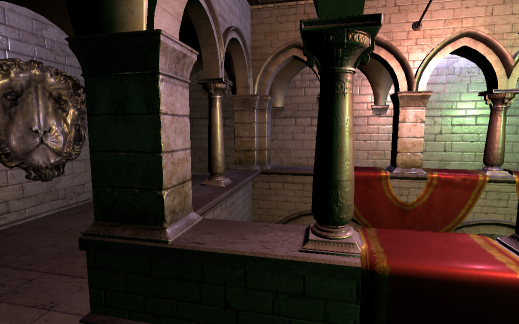
\includegraphics[width=0.4\linewidth]{./Chapters/linearOptScr1.jpg}}
  \subfigure{\label{fig:linFuncOpt2}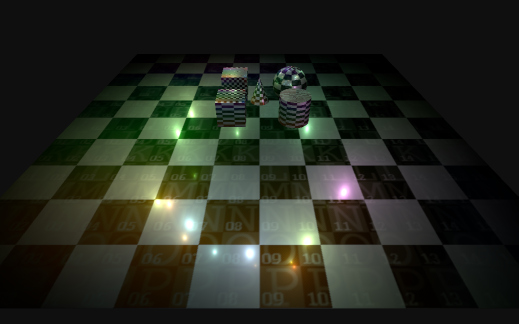
\includegraphics[width=0.4\linewidth]{./Chapters/linearOptScr2.jpg}}
  \caption{Scenes used to test the speedup from optimization due to linear functions}
  \label{fig:linFuncOpt}
\end{figure}

Figure \ref{fig:linFuncOpt} shows two scenes, which render respectively at 93 and 131 FPS without the optimization step. With it enabled, the performance reaches 96 FPS and 133 FPS respectively.

\subsection{Code generation for functional composition}

TODO: Describe what functional composition turns into
